\section{Visibilidade}
\label{s.visibility}

\subsection{O que é?}
\label{ss.what_visibility}

\begin{frame}{O que é?}
	\justify 
	\begin{itemize}
		\item<1> Do latim \textit{visibilitas}, visibilidade é a qualidade/estado do que é visível;
		\\~\\
		\item<2> Ser/estar \textbf{visível} é um \textbf{conceito} muito \textbf{amplo} e depende de inúmeros fatores, tais como, área de pesquisa, impacto social, dentre outros;
		\\~\\
		\item<3> Como é possível \textbf{mensurar} a \textbf{visibilidade} de uma pesquisa?
	\end{itemize}
\end{frame}

\begin{frame}{}
	\centering
	\begin{figure}
		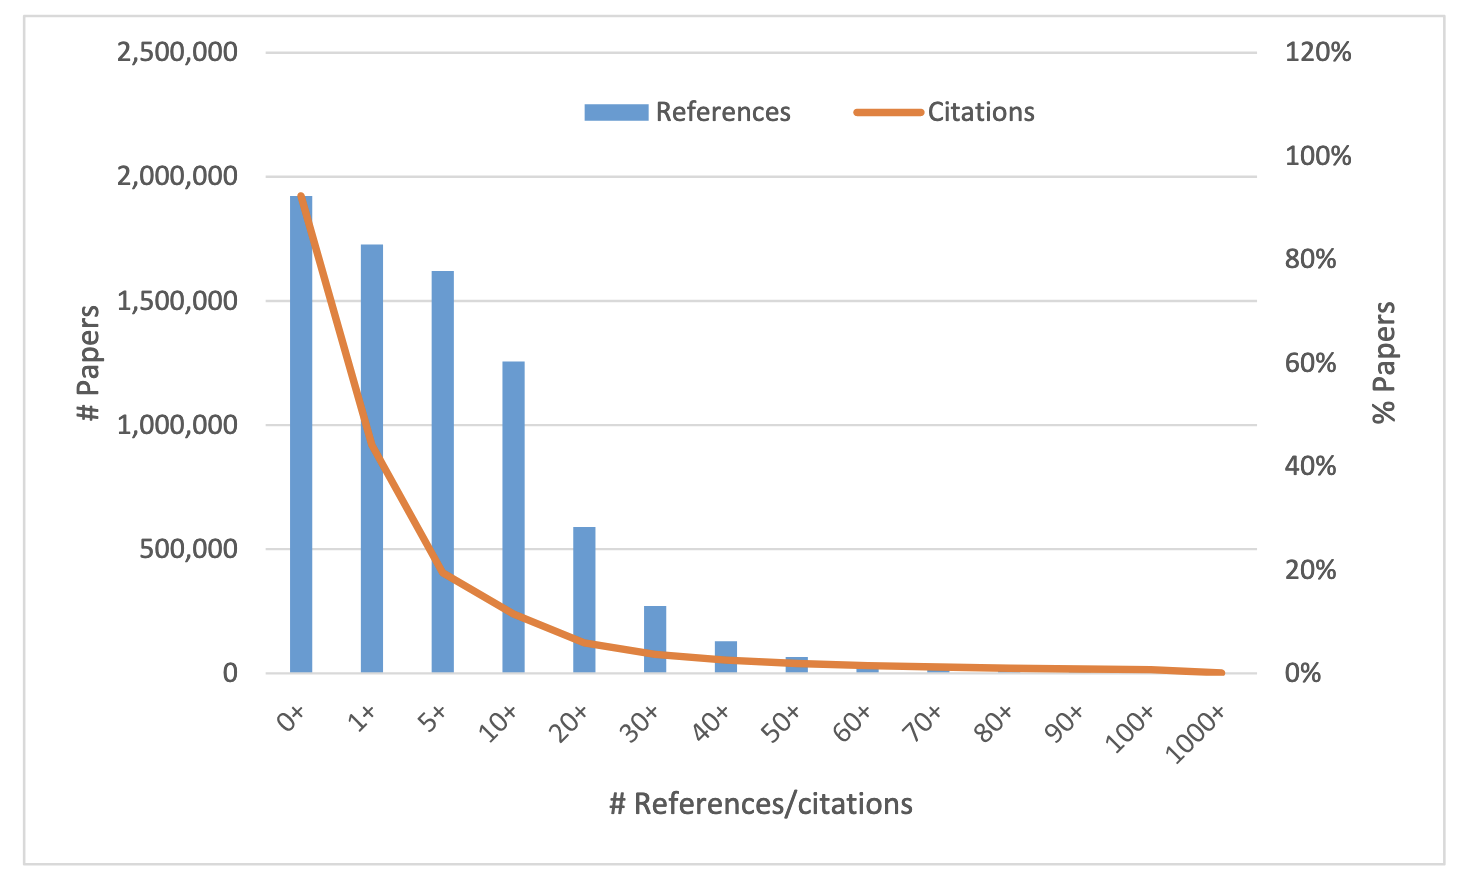
\includegraphics[scale=0.375]{figs/citations_per_paper.png}
		\caption{Distribuição do número de referências e citações por artigo~\cite{Fiala:17}.}
		\label{f.citations_per_paper}
	\end{figure}	
\end{frame}

\subsection{Por que investir?}
\label{ss.why_visibility}

\begin{frame}{Por que investir?}
	\justify 
	\begin{itemize}
		\item<1> Ampliar o \textbf{alcance} e o possível \textbf{impacto social} da pesquisa;
		\\~\\
		\item<2> ``Expor"~o \textbf{nome} da \textbf{universidade} em que a pesquisa foi conduzida;
		\\~\\
		\item<3> Possibilitar a \textbf{colaboração} com pesquisadores de outras universidades e centros de pesquisa;
		\\~\\
		\item<4> \textbf{Mérito} pessoal, \textbf{aspirações} profissionais, dentre outros.
	\end{itemize}
\end{frame}

\begin{frame}{}
	\centering
	\begin{figure}
		
\includegraphics[scale=0.2]{figs/keras.png}
		\caption{A biblioteca Keras~\cite{Chollet:15}, desenvolvida por François Chollet, foi incorporada ao Tensorflow e o autor contratado pela Google.}
		\label{f.keras}
	\end{figure}
\end{frame}


\subsection{Como ampliar?}
\label{ss.how_visibility}

\begin{frame}{Como ampliar?}
	\justify 
	\begin{itemize}
		\item<1> Exposição de \textbf{pré-publicação} e/ou \textbf{código aberto} relacionado à pesquisa;
		\\~\\
		\item<2> \textbf{Documentação} para terceiros conseguirem reproduzir a pesquisa;
		\\~\\
		\item<3> \textbf{Manutenção} e disponibilidade para responder dúvidas e auxiliar usuários em utilizar a pesquisa;
		\\~\\
		\item<4> \textbf{Divulgação} da pesquisa em redes sociais e/ou locais pertinentes.
	\end{itemize}
\end{frame}